\documentclass[10pt]{standalone}

\input{../tikzpic_packages.tex}


\begin{document}
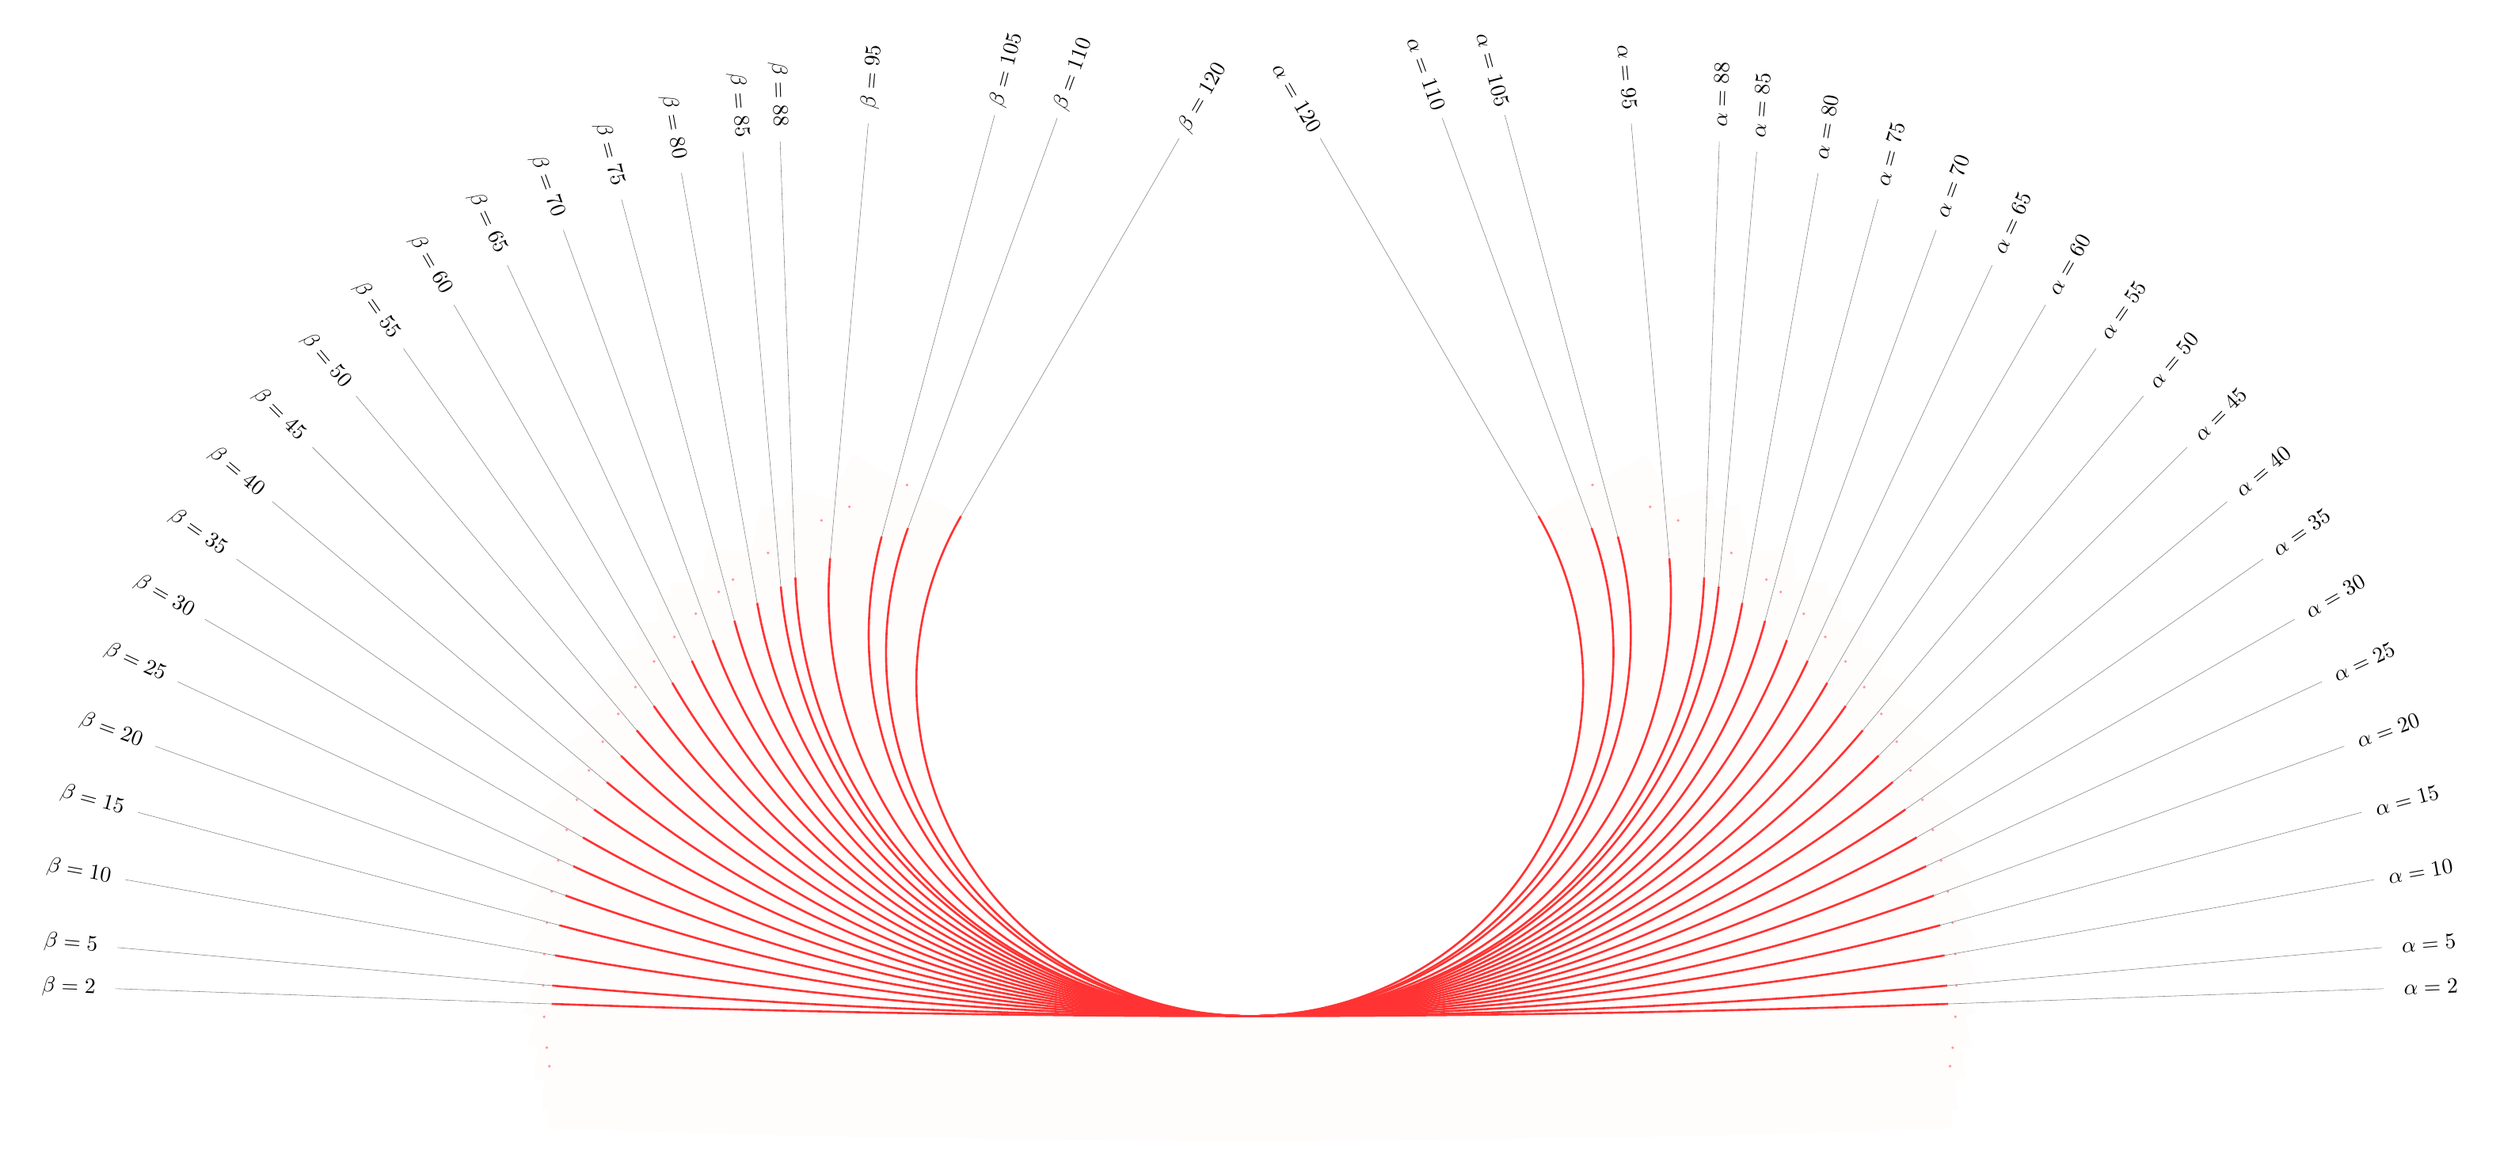
\begin{tikzpicture}[
scale=1, 
stretch/.style={color=red!1, line width=2cm},
%dstretch/.style={color=red!40, line width=1.333cm},
foot/.style={fill=red!10, line width=.333mm, draw=red!40},
solid/.style={line width=.333mm, draw=red!80},
help/.style={very thin, lightgray},
arrow/.style={triangle 45-}
]

%% Box
%\path[clip](-20.5,17.5)rectangle(43,-3.5);

\def\hx{11.2}	% length of legs
\def\hy{2}  % change only with line width of stretch
\def\rf{.0003}	% radius of foot
\pgfmathsetmacro{\rfh}{\rf*.5}
\pgfmathsetmacro{\hyh}{.5*\hy}
\pgfmathsetmacro{\hxh}{\hx/2}



\foreach \alp in {120,110,105,95,88,85,80,75,70,65,60,55,50,45,40,35,30,25,20,15,10,5,2}{

\def\bet{\alp}

\def\pi{3.1416}
\pgfmathsetmacro{\r}{\hx/\alp*180/\pi}
\pgfmathsetmacro{\rb}{\hx/\bet*180/\pi}

% % Links
\draw[stretch] (0,0)arc(270:270-\bet:\rb+\hyh)++(-\bet+180:\rfh) coordinate(X);
\draw[solid] (-90:-\hyh)coordinate(O)arc(270:270-\bet:\rb)coordinate(help);

\draw[help lines] (help)--++(-\bet+180:7)coordinate(help);
\path (help)--++(-\bet+180:1.5)node[midway,sloped]{$\beta = \bet$};
\draw[foot] (X) circle(\rf);

% % Rechts
\draw[stretch] (0,0)arc(270:270+\alp:\r+\hyh) ++(\alp:\rfh)coordinate(X);
\draw[solid] (-90:-\hyh)arc(270:270+\alp:\r)coordinate(help);

\draw[help lines] (help)--++(\alp:7)coordinate(help);
\path (help)--++(\alp:1.5)node[midway,sloped]{$\alpha = \alp$};
\draw[foot] (X) circle(\rf);
}





\end{tikzpicture}
\end{document}